\documentclass{beamer}
\usetheme{Darmstadt}
\usepackage{comment}
\usepackage[utf8]{inputenc}    % Para escribir acentos y caracteres especiales
\usepackage{graphicx}          % Para insertar imágenes
\usepackage{booktabs}          % Para tablas más bonitas
\usepackage{enumitem}
\usepackage{amsmath}           % Para escribir ecuaciones
\usepackage{tikz}              % Para gráficos vectoriales
\usetikzlibrary{arrows.meta, positioning}
\usetikzlibrary{calc}          % Para coordenadas calculadas con TikZ
\usepackage{pgfplots}          % Para gráficos matemáticos
\pgfplotsset{compat=1.18}      % Evita errores por compatibilidad
\usepackage{hyperref}
\usepackage{pgf}
\usepackage{ragged2e}

\newif\ifpresentacion
\ifdefined\versionpresentacion
  \edef\tempver{\versionpresentacion}
  \ifx\tempver\empty
    \presentacionfalse
  \else
    \ifnum\pdfstrcmp{\tempver}{true}=0
      \presentaciontrue
    \else
      \presentacionfalse
    \fi
  \fi
\else
  \presentacionfalse
\fi

\usepackage{ifthen}
\newcommand{\pausa}{\ifpresentacion\pause\fi}
% #region Título
\title{Ayudantía 4 \\  Árboles Binomiales
\\ \large\textit{Instrumentos Derivados}}
\author{
  \texorpdfstring{
    \textbf{Profesor:} Francisco Rantul \\[0.3em]
    \textbf{Ayudante:} Mateo Canales
  }{Profesor: Francisco Rantul, Ayudante: Mateo Canales}
}
\subject{Instrumentos Derivados}
\institute{Universidad Diego Portales}
\date{04 De Junio, 2025}
% #endregion 
\begin{document}

% Portada
\begin{frame}
    \titlepage
    \vfill
    \centering
    
\includegraphics[width=2.3118cm]{../imagenes/logo.png}
  \end{frame}

% #region Formateo de números 
\newcommand{\cajaverde}[1]{%
  \fcolorbox{blue}{green!20}{%
    { #1}%
  }
}
\newcommand{\cajaverdeletra}[1]{%
  \fcolorbox{blue}{green!20}{%
    \parbox{0.9\linewidth}{\justifying #1}%
  }
}
\newcommand{\formula}[1]{\textcolor{blue}{#1}}
\newcommand{\entero}[1]{\pgfmathprintnumber[fixed, precision=0]{#1}}
\newcommand{\decimal}[1]{\pgfmathprintnumber[fixed, precision=2]{#1}}
\newcommand{\decimalx}[1]{\pgfmathprintnumber[fixed, precision=3]{#1}}
\newcommand{\decimalxx}[1]{\pgfmathprintnumber[fixed, precision=4]{#1}}
\newcommand{\porcentaje}[1]{%
  \pgfmathsetmacro{\temp}{#1*100}%
  \pgfmathprintnumber[fixed, precision=2]{\temp}\%%
  }
\newcommand{\dinero}[1]{%
  \$\,\pgfmathprintnumber[fixed, precision=0]{#1}
  }
\newcommand{\dineros}[1]{%
  \$\,\pgfmathprintnumber[fixed, precision=1]{#1}
  }
\newcommand{\Desarrollo}[1]{Desarrollo Parte {#1})}
% #endregion

% Pregunta 1)

\section{Pregunta 1}

% #region Variables pregunta 1
\newcommand{\Kuno}{100}
\newcommand{\diezp}{0.1}
\newcommand{\ochop}{0.08}
\newcommand{\semestre}{0.5}
% Fórmulas
\newcommand{\arbol}{$p = \frac{e^{r\cdot \Delta t}-d}{u-d}$}
\newcommand{\neutral}{$f = e^{-r \cdot \Delta t}\cdot (p \cdot f_u+(1-p) \cdot f_d)$}
\newcommand{\putcall}{$S_0+p = K \cdot e^{-r \cdot T}+c$}
\newcommand{\ceroud}{$S_0u|d=S_0*(1+(subida|bajada)) $}
% Preguntas
\newcommand{\Preguno}{ El precio de una acción es de \dinero{\Kuno}. En 6 meses más se espera que suba o baje un \porcentaje{\diezp}. La tasa libre de riesgo es del \porcentaje{\ochop} anual continua. } 
\newcommand{\Pregunoa}{¿Cuál es el valor de una opción call europea de 1 año con strike Price $ K = \dinero{\Kuno} $?}
\newcommand{\Pregunob}{¿Cuál es el valor de una opción put europea de 1 año con strike Price $ K = \dinero{\Kuno} $?}
\newcommand{\Pregunoc}{Verifique que se cumple la paridad Put-Call}
\newcommand{\Uuno}{1.1}
\newcommand{\Duno}{0.9}

\pgfmathsetmacro{\uno}{exp(\ochop*\semestre)}
\pgfmathsetmacro{\dos}{\uno-\Duno}
\pgfmathsetmacro{\dosa}{\Uuno-\Duno}
\pgfmathsetmacro{\tres}{\dos/\dosa}
\pgfmathsetmacro{\scerod}{\Kuno*\Duno}
\pgfmathsetmacro{\scerodd}{\Kuno*\Duno*\Duno}
\pgfmathsetmacro{\scerou}{\Kuno*\Uuno}
\pgfmathsetmacro{\scerouu}{\Kuno*\Uuno*\Uuno}
\pgfmathsetmacro{\scerodu}{\Kuno*\Uuno*\Duno}
\pgfmathsetmacro{\fcerodd}{\scerodd-\Kuno}
\pgfmathsetmacro{\fcerodu}{\scerodu-\Kuno}
\pgfmathsetmacro{\fcerouu}{\scerouu-\Kuno}
\pgfmathsetmacro{\fceroputdd}{\Kuno-\scerodd}
\pgfmathsetmacro{\fceroputdu}{\Kuno-\scerodu}
\pgfmathsetmacro{\fceroputuu}{\Kuno-\scerouu}

\pgfmathsetmacro{\cuatrou}{exp(-\ochop*\semestre)*(\tres*\fcerouu)}
\pgfmathsetmacro{\cuatro}{exp(-\ochop*\semestre)*(\tres*\cuatrou)}
\pgfmathsetmacro{\cincou}{exp(-\ochop*\semestre)*((1-\tres)*\fceroputdu)}
\pgfmathsetmacro{\cincod}{exp(-\ochop*\semestre)*(\tres*\fceroputdu+(1-\tres)*\fceroputdd)}
\pgfmathsetmacro{\cinco}{exp(-\ochop*\semestre)*(\tres*\cincou+(1-\tres)*\cincod)}
\pgfmathsetmacro{\seis}{\Kuno+\cinco}
\pgfmathsetmacro{\seisa}{\Kuno * exp(-\ochop)+ \cuatro}

% #endregion 

% Presentacion de preguntas 1
\begin{frame}
  \frametitle{Pregunta 1}
  \justify
  \Preguno 

    \vspace{1em}

    \begin{enumerate}[label=\textbf{\alph*)}]
      \item \Pregunoa
      \item \Pregunob
      \item \Pregunoc
  \end{enumerate}
\end{frame}

%presentacion de preguntas 1 y recopilación de datos
\subsection{Parte a)}

\begin{frame}{Pregunta 1 Parte a)}
  \justify
  \Preguno
  \vspace{1em}
  
  \textbf{a)}  \Pregunoa
  
\end{frame}
  

\begin{frame}{\Desarrollo{a}}
  Valor de la acción\\
    $S_0=\dinero{\Kuno}$\\  \pausa
    $S_0d=\Kuno \cdot \Duno \pausa = \dinero{\scerod}$\\  \pausa
    $S_0u=\Kuno \cdot \Uuno \pausa = \dinero{\scerou}$\\  \pausa
    $S_0d^2=\Kuno \cdot \Duno \cdot \Duno\pausa = \dinero{\scerodd}$\\  \pausa
    $S_0du=\Kuno \cdot \Duno \cdot \Uuno\pausa = \dinero{\scerodu}$\\  \pausa
    $S_0u^2=\Kuno \cdot \Uuno \cdot \Uuno\pausa = \dinero{\scerouu}$\\ \pausa
  Valor de la opción:\\ 
    $f_{dd}=\max[\decimal{\scerodd}-\Kuno , 0]\pausa=\max[\decimal{\fcerodd}, 0]$\\\pausa
    $f_{dd}=0$\\\pausa
    $f_{du}=\max[\decimal{\scerodu}-\Kuno , 0]\pausa=\max[\decimal{\fcerodu}, 0]$\\\pausa
    $f_{du}=0$\\\pausa
    $f_{uu}=\max[\decimal{\scerouu}-\Kuno , 0]\pausa=\max[\decimal{\fcerouu}, 0]$\\\pausa
    $f_{uu}=\decimal{\fcerouu}$\\
 
\end{frame}

\begin{frame}{\Desarrollo{a}}
  Datos: $u = \Uuno$, $d = \Duno$, $\Delta_t=\semestre$, $r = \ochop$.\\
    \pausa 
    \textbf{Fórmula :} \formula{\arbol}  \\
    \pausa
    Desarrollando la fórmula:\\
    $p = \frac{e^{\ochop \cdot \semestre}-\Duno}{\Uuno-\Duno}$
    \pausa
    \\
    $p = \frac{\decimalx{\dos}}{\decimalx{\dosa}}$
    \\
    \pausa
    $p = \decimalx{\tres}$
    \\
    \pausa
  Usamos la fórmula neutral al riesgo\\
  \textbf{Fórmula :} \formula{\neutral}  \\\pausa
    $f_u=e^{-\ochop \cdot \semestre}(\decimalx{\tres} \cdot \decimal{\fcerouu}+(1-\decimalx{\tres}) \cdot 0)\pausa = \decimalx{\cuatrou}$\\\pausa
    $f_d=e^{-\ochop \cdot \semestre}(\decimalx{\tres} \cdot 0+(1-\decimalx{\tres}) \cdot 0)\pausa = 0$\\\pausa
    $f=e^{-\ochop \cdot \semestre}(\decimalx{\tres} \cdot \decimalx{\cuatrou}+(1-\decimalx{\tres}) \cdot 0)\pausa = \decimalx{\cuatro}$\\\pausa
  \cajaverde{$f=\decimalx{\cuatro}$}
\end{frame}

\begin{comment}
  
\begin{frame}{Árbol binomial simple}
  \centering
  \begin{tikzpicture}[
    every node/.style={font=\tiny, inner sep=2pt},
    dot/.style={circle,fill=black,minimum size=3pt,inner sep=0pt},
    >=Stealth
  ]
  
  % Nodos
  \node (S0) at (0,0) {}; % Punto
  \node[dot, label=left:$\begin{aligned} S_0= \\ f=\decimalx{\cuatro} \end{aligned}$] at (S0) {};  % Etiqueta
  
  \node (Su) at (2,1) {};% Punto
  \node[dot, label=above:$\begin{aligned} S_0u= \\ f_u=\decimalx{\cuatrou}  \end{aligned}$] at (Su) {}; % Etiqueta
  \draw[->] (S0) -- (Su);% Flecha
  
  \node (Sd) at (2,-1) {};% Punto
  \node[dot, label=below:$\begin{aligned} S_0d \\ f_d=0  \end{aligned}$] at (Sd) {}; % Etiqueta
  \draw[->] (S0) -- (Sd); % Flecha
  
  \node (Sdu) at (4,0) {};% Punto
  \node[dot, label=right:$\begin{aligned} S_0du \\ f_du=  \end{aligned}$] at (Sdu) {}; % Etiqueta
  \draw[->] (Sd) -- (Sdu); % Flecha
  \draw[->] (Su) -- (Sdu); % Flecha
  
  \node (Sdd) at (4,-2) {};% Punto
  \node[dot, label=right:$\begin{aligned} S_0dd \\ f_dd=  \end{aligned}$] at (Sdd) {}; % Etiqueta
  \draw[->] (Sd) -- (Sdd); % Flecha
  
  \node (Suu) at (4,2) {};% Punto
  \node[dot, label=right:$\begin{aligned} S_0uu \\ f_uu=  \end{aligned}$] at (Suu) {}; % Etiqueta
  \draw[->] (Su) -- (Suu);% Flecha
  
  \end{tikzpicture}
  \end{frame}
\end{comment}

\subsection{Parte b)}

\begin{frame}{Pregunta 1 Parte b)}
  \justify
  \Preguno
  \vspace{1em}
  
  \textbf{a)}  \Pregunob
  
\end{frame}

\begin{frame}{\Desarrollo{b}}
  Valor de la opción:\\ 
    $f_{dd}=\max[\Kuno-\decimal{\scerodd} , 0]\pausa=\max[\decimal{\fceroputdd}, 0]$\\\pausa
    $f_{dd}=\decimal{\fceroputdd}$\\\pausa
    $f_{du}=\max[\Kuno-\decimal{\scerodu} , 0]\pausa=\max[\decimal{\fceroputdu}, 0]$\\\pausa
    $f_{du}=\decimal{\fceroputdu}$\\\pausa
    $f_{uu}=\max[\Kuno-\decimal{\scerouu} , 0]\pausa=\max[\decimal{\fceroputuu}, 0]$\\\pausa
    $f_{uu}=0$\\
    Usamos la fórmula neutral al riesgo\\
    \textbf{Fórmula :} \formula{\neutral}  \\\pausa
      $f_u=e^{-\ochop \cdot \semestre}(\decimalx{\tres} \cdot 0+(1-\decimalx{\tres}) \cdot \decimal{\fceroputdu})\pausa = \decimalx{\cincou}$
      $f_d=e^{-\ochop \cdot \semestre}(\decimalx{\tres} \cdot \decimal{\fceroputdu}+(1-\decimalx{\tres}) \cdot \decimal{\fceroputdd})\pausa = \decimalx{\cincod}$
      $f=e^{-\ochop \cdot \semestre}(\decimalx{\tres} \cdot \decimalx{\cincou}+(1-\decimalx{\tres}) \cdot \decimalx{\cincod})\pausa = \decimalx{\cinco}$
      \cajaverde{$f=\decimalx{\cinco}$}
 
\end{frame}

\subsection{Parte c)}

\begin{frame}{Pregunta 1 Parte c)}
  \justify
  \Preguno
  \vspace{1em}
  
  \textbf{a)}  \Pregunoc
  
\end{frame}

\begin{frame}{\Desarrollo{c}}
La paridad Put-call se define como:   \\
 \formula{\putcall}  \\\pausa
 El valor de la acción más el precio de la put es:\\
 $\Kuno + \decimalx{\cinco} \pausa = \decimalx{\seis}$\pausa\\
 El valor presente del strike Price más el precio de la call es:\\
$\Kuno \cdot e^{-\ochop \cdot 1}+ \decimalx{\cuatro}=\decimalx{\seisa}$\\\pausa
 \vspace{1em|}
  \cajaverdeletra{
  En este caso se puede ver que existe diferencia entre ambos cálculos,
  sin embargo, esto se debe  al los decimales utilizados, pero, si lo ingresamos 
  directamente en la calculadora, se cumple la paridad. 
  }
  
\end{frame}

\section{Pregunta 2}

% #region Variables pregunta 2
\newcommand{\pdos}{50}
\newcommand{\pdosu}{53}
\newcommand{\pdosd}{48}
\newcommand{\Kdos}{49}
\pgfmathsetmacro{\fdosd}{\pdosd-\Kdos}
\pgfmathsetmacro{\fdosu}{\pdosu-\Kdos}
\pgfmathsetmacro{\Sdelta}{\pdosu-\pdosd}
\pgfmathsetmacro{\deltados}{\fdosu/\Sdelta}
\pgfmathsetmacro{\xdosu}{\pdosu*\deltados-\fdosu}
\pgfmathsetmacro{\xdosd}{\pdosd*\deltados}
\pgfmathsetmacro{\tdos}{2/12}
\pgfmathsetmacro{\runo}{\pdos*\deltados}
\pgfmathsetmacro{\rdos}{\pdosu*\deltados}
\pgfmathsetmacro{\rtres}{exp(-\diezp*\tdos)}
\pgfmathsetmacro{\rcuatro}{\rdos-\fdosu}
\pgfmathsetmacro{\rcinco}{\rcuatro*\rtres}
\pgfmathsetmacro{\rseis}{\rcinco - \runo}
\pgfmathsetmacro{\rsiete}{-\rseis}
\pgfmathsetmacro{\ccero}{exp(\diezp*\tdos)}
\pgfmathsetmacro{\cuno}{\pdosu/\pdos}
\pgfmathsetmacro{\cdos}{\pdosd/\pdos}
\pgfmathsetmacro{\ctres}{\cuno-\cdos}
\pgfmathsetmacro{\ccuatro}{\ccero-\cdos}
\pgfmathsetmacro{\ccinco}{\ccuatro/\ctres}
\pgfmathsetmacro{\cseis}{\ccinco*\fdosu}
\pgfmathsetmacro{\csiete}{(1-\ccinco)}
\pgfmathsetmacro{\cocho}{\rtres*\cseis}



% Preguntas
\newcommand{\Pregdos}{El precio de una acción es de \dinero{\pdos}. 
En 2 meses más podría valer \dinero{\pdosu} o \dinero{\pdosd}. La tasa libre de riesgo es del \porcentaje{\diezp}
anual continua. Calcule el valor de una opción call europea de 2 meses con strike Price K=\dinero{\Kdos}. 
Considere un árbol de un solo paso. }
\newcommand{\Pregdosa}{Valorice la opción call europea usando argumentos de no arbitraje. }
\newcommand{\Pregdosb}{Valorice la opción call europea usando probabilidades neutrales al riesgo. }

% Fórmulas
\newcommand{\neutrali}{$S_0d\cdot \Delta-f_d=S_0u\cdot \Delta-f_u$}
\newcommand{\portafolio}{$S_0\cdot \Delta-f=(S_0u\cdot \Delta-f_u) \cdot e^{-rT}$}
\newcommand{\calcud}{$u|d=\frac{S_0u|d}{S_0}$}
% #endregion

% Pregunta 2

\begin{frame}{Pregunta 2}
  \justify
\Pregdos
\vspace{1em}

\begin{enumerate}[label=\textbf{\alph*)}]
  \item \Pregdosa
  \item \Pregdosb
\end{enumerate}

\end{frame}
  
\subsection{Parte a)}

\begin{frame}{Pregunta 2 Parte a)}
  \justify
  
  \Pregdos\\

  \vspace{1em}
  \textbf{a)} \Pregdosa
\end{frame}
  
\begin{frame}{\Desarrollo{a}}
 Los posibles valores de la acción son $S_{0u}=\pdosu$, $S_{0f}=\pdosd$.
\pausa
  Por ende los posibles valores de la opción son: 
 $f_{d}=\max[\decimal{\pdosd}-\Kdos , 0]\pausa=\max[\decimal{\fdosd}, 0]$\\\pausa
 $f_{d}=0$\\\pausa
 $f_{u}=\max[\decimal{\pdosu}-\Kdos , 0]\pausa=\max[\decimal{\fdosu}, 0]$\\\pausa
 $f_{d}=\decimal{\fdosu}$\\\pausa
 Asumamos un portafolio de $+ \Delta$ acciones y una posición corta en una opción $-f$\\
 Usaremos la fórmula: \\
 \formula{\neutrali}\\\pausa
 {$\decimal{\pdosd}\cdot \Delta-0=\decimal{\pdosu}\cdot \Delta-\decimal{\fdosu}$}\\\pausa
 {$(\decimal{\pdosd}-\decimal{\pdosu})\cdot \Delta=-\decimal{\fdosu}$}\\\pausa
 {$\decimal{\Sdelta}\cdot \Delta=\decimal{\fdosu}$}\\\pausa
 {$\Delta=\frac{\decimal{\fdosu}}{\decimal{\Sdelta}}$}\\\pausa
 \cajaverde{$\Delta=\decimalx{\deltados}$}


\end{frame}

\begin{frame}{\Desarrollo{a}}
  En $T= \frac{2}{12}$ el valor de los portafolios pesimistas y optimistas son:\\
  $f_d=\decimal{\pdosd}\cdot \Delta-0\pausa=\decimal{\pdosd}\cdot\decimalx{\deltados}\pausa=\decimal{\xdosd}$\\\pausa
  $f_u=\decimal{\pdosu}\cdot \Delta-\decimalx{\fdosu}\pausa=\decimal{\pdosu}\cdot\decimalx{\deltados}-\decimal{\fdosu}\pausa=\decimal{\xdosu}$\\\pausa
  Se comprueba que el portafolio tendrá un comportamiento idéntico en ambos casos.\\
  Teniendo en cuenta todo lo anterior, ahora podemos valorizar la opción con la fórmula en que 
  el valor presente de la accion es igual al costo de construirla.\\\pausa
  \formula{\portafolio}\\
  Con los datos: $S_0= \pdos$, $\Delta=\decimal{\deltados}$, $S_0u=\decimal{\pdosu}$, $f_u=\decimal{\fdosu}$, 
  $r=\decimal{\diezp}$,$T=\frac{2}{12}=\decimalx{\tdos}$\\
\end{frame}

\begin{frame}{\Desarrollo{a}}
  \formula{\portafolio}\\
  Con los datos: $S_0= \pdos$, $\Delta=\decimal{\deltados}$, $S_0u=\decimal{\pdosu}$, $f_u=\decimal{\fdosu}$, 
  $r=\decimal{\diezp}$,$T=\frac{2}{12}=\decimalx{\tdos}$\\
  Reemplazamos:\\
  $\pdos \cdot \decimal{\deltados} - f=(\decimal{\pdosu}\cdot \decimal{\deltados}-\decimal{\fdosu}) 
  \cdot e^{\decimal{\diezp}\cdot\decimalx{\tdos}} $\\\pausa
  $\decimal{\runo}-f=(\decimal{\rdos}-\decimal{\fdosu})\cdot \decimal{\rtres}$\\\pausa
  $-f=(\decimal{\rcuatro})\cdot \decimal{\rtres}-\decimal{\runo}$\\\pausa
  $-f=\decimal{\rcinco}-\decimal{\runo}$\\\pausa
  $-f=\decimalx{\rseis}$\\\pausa
  \cajaverde{$f=\decimalx{\rsiete}$}\\\pausa
  
\end{frame}

\subsection{Parte b)}

\begin{frame}{Pregunta 2 Parte b)}
  \justify
  
  \Pregdos\\
  
  \vspace{1em}
  \textbf{b)} \Pregdosb
\end{frame}
  
\begin{frame}{\Desarrollo{b}}
Calculamos u y d, según la fórmula\\
\formula{\calcud}\\
$u=\frac{\pdosu}{\pdos}\pausa = \decimalx{\cuno}$\\\pausa
\vspace{.5em}
$d=\frac{\pdosd}{\pdos}\pausa =\decimalx{\cdos}$\\\pausa
Ahora usamos la fórmula de probabilidad:
\formula{\arbol}\\\pausa
Datos $r=\diezp$, $T=\frac{2}{12}=\decimalx{\tdos}$, $u=\decimalx{\cuno}$, $d=\decimalx{\cdos}$\\\pausa
$p = \frac{e^{\diezp \cdot \decimalx{\tdos}}-\decimalx{\cdos}}{\decimalx{\cuno}-\decimalx{\cdos}}$\\\pausa
$p = \frac{\decimalx{\ccero}-\decimalx{\cdos}}{\decimalx{\ctres}}$\\\pausa
$p = \frac{\decimalx{\ccuatro}}{\decimalx{\ctres}}$\\\pausa
\cajaverde{$p=\decimalx{\ccinco}$}\\\pausa
\end{frame}
\begin{frame}{\Desarrollo{b}}
Teniendo estos datos, podemos reemplazar enla fórmula neutral al riesgo.\\
  \formula{\neutral}\\
  $f = e^{-\diezp \cdot \decimalx{\tdos}}\cdot (\decimalx{\ccinco}\cdot \decimal{\fdosu}+(1-\decimalx{\ccinco}) \cdot 0)$\\\pausa
  $f = \decimalx{\rtres} \cdot (\decimalx{\cseis}+(\decimalx{\csiete}) \cdot 0)$ \\\pausa
  $f = \decimalx{\rtres} \cdot (\decimalx{\cseis}+ 0)$\\\pausa
  $f = \decimalx{\rtres} \cdot (\decimalx{\cseis})$\\\pausa
  \cajaverde{$f = \decimalx{\cocho}$}\\\pausa
\end{frame}

\section{Pregunta 3}

  
% #region Variables Pregunta 3
\newcommand{\stres}{40}
\newcommand{\trimestre}{0.25}
\newcommand{\docep}{0.12}
\newcommand{\ktres}{42}
\newcommand{\Dtres}{0.9}
\newcommand{\Utres}{1.1}

\pgfmathsetmacro{\stresd}{\stres*\Dtres}
\pgfmathsetmacro{\stresdd}{\stres*\Dtres*\Dtres}
\pgfmathsetmacro{\stresu}{\stres*\Utres}
\pgfmathsetmacro{\stresuu}{\stres*\Utres*\Utres}
\pgfmathsetmacro{\stresdu}{\stres*\Utres*\Dtres}

\pgfmathsetmacro{\ftresuu}{\ktres-\stresuu}
\pgfmathsetmacro{\ftresdu}{\ktres-\stresdu}
\pgfmathsetmacro{\ftresdd}{\ktres-\stresdd}
\pgfmathsetmacro{\ftresuj}{ \ktres-\stresu }  
\pgfmathsetmacro{\ftresdj}{ \ktres-\stresd }
\pgfmathsetmacro{\ftresj}{ \ktres-\stres }


\pgfmathsetmacro{\ftresuum}{max(\ftresuu,0)}
\pgfmathsetmacro{\ftresdum}{max(\ftresdu,0)}
\pgfmathsetmacro{\ftresddm}{max(\ftresdd,0)}
\pgfmathsetmacro{\ftresum}{ max(\ftresuj,0)}
\pgfmathsetmacro{\ftresdm}{ max(\ftresdj,0)}
\pgfmathsetmacro{\ftresm}{ max(\ftresj,0)}



\pgfmathsetmacro{\tuno}{exp(\docep*\trimestre)}
\pgfmathsetmacro{\tdos}{\tuno-\Dtres}
\pgfmathsetmacro{\tdosa}{\Utres-\Dtres}
\pgfmathsetmacro{\ttres}{\tdos/\tdosa}

\pgfmathsetmacro{\ftresu}{exp(-\docep*\trimestre)*(\ttres*\ftresuum+(1-\ttres)*\ftresdum)}
\pgfmathsetmacro{\ftresd}{exp(-\docep*\trimestre)*(\ttres*\ftresdum+(1-\ttres)*\ftresddm)}
\pgfmathsetmacro{\ftres}{exp(-\docep*\trimestre)*(\ttres*\ftresu+(1-\ttres)*\ftresd)}

\pgfmathsetmacro{\ftresdf}{ max({\ftresdm},{\ftresd})}
\pgfmathsetmacro{\ftresuf}{ max({\ftresum},{\ftresu})}
\pgfmathsetmacro{\ftresk}{exp(-\docep*\trimestre)*(\ttres*\ftresuf+(1-\ttres)*\ftresdf)}
\pgfmathsetmacro{\ftresf}{ max({\ftresm},{\ftresk})}

% Preguntas

\newcommand{\Pregtres}{
  El precio de una acción es de \dinero{\stres}. Cada 3 meses se espera que suba o baje un \porcentaje{\diezp}.
  La tasa libre de riesgo es de \porcentaje{\docep} anual continua.}
\newcommand{\Pregtresa}{Calcule el valor de una opción put europea a 6 meses con strike Price $K=\ktres$.}
\newcommand{\Pregtresb}{Calcule una opción put americana a 6 meses con strike Price $K=\ktres$.}
\newcommand{\Pregtresc}{Explique la razón en la diferencia del valor respecto a la opción europea.}
% Fórmulas

% #endregion
\begin{frame}{Pregunta 3}
  \justify
\Pregtres
\vspace{1em}

\begin{enumerate}[label=\textbf{\alph*)}]
  \item \Pregtresa
  \item \Pregtresb
  \item \Pregtresc
\end{enumerate}

\end{frame}

\subsection{Parte a)}

\begin{frame}{Pregunta 3 Parte a)}
  \justify
  
  \Pregtres\\

  \vspace{1em}
  \textbf{a)} \Pregtresa
\end{frame}

\begin{frame}{\Desarrollo{a}}
  Sabemos que en un periodo, la acción puede bajar o subir \porcentaje{\diezp}.\\
  Valor de la acción\\
  $S_0=\dineros{\stres}$\\  \pausa
  $S_0d=\stres \cdot \Dtres \pausa = \dineros{\stresd}$\\ \pausa
  $S_0u=\stres \cdot \Utres \pausa = \dineros{\stresu}$\\  \pausa
  $S_0d^2=\stres \cdot \Dtres \cdot \Dtres\pausa = \dineros{\stresdd}$\\  \pausa
  $S_0du=\stres \cdot \Dtres \cdot \Utres\pausa = \dineros{\stresdu}$\\  \pausa
  $S_0u^2=\stres \cdot \Utres \cdot \Utres\pausa = \dineros{\stresuu}$\\  \pausa
  Valor de la opción:\\ 
  $f_{dd}=\max[\ktres-\decimal{\stresdd} , 0]\pausa=\max[\decimal{\ftresdd}, 0]$\\\pausa $f_{dd}=\decimal{\ftresddm}$\\\pausa
  $f_{du}=\max[\ktres-\decimal{\stresdu} , 0]\pausa=\max[\decimal{\ftresdu}, 0]$\\\pausa $f_{du}=\decimal{\ftresdum}$\\\pausa
  $f_{uu}=\max[\ktres-\decimal{\stresuu} , 0]\pausa=\max[\decimal{\ftresuu}, 0]$\\\pausa $f_{uu}=\decimal{\ftresuum}$\\
\end{frame}

\begin{frame}{\Desarrollo{a}}
  Datos: $u = \Utres$, $d = \Dtres$, $\Delta_t=\trimestre$, $r = \docep$.\\ \pausa 
    \textbf{Fórmula :} \formula{\arbol}  \\ \pausa
    Desarrollando la fórmula:\\
    $p = \frac{e^{\docep \cdot \trimestre}-\Dtres}{\Utres-\Dtres}$\\    \pausa
    $p = \frac{\decimalx{\tdos}}{\decimalx{\tdosa}}$\\    \pausa
    $p = \decimalx{\ttres}$\\    \pausa
  Usamos la fórmula neutral al riesgo\\
  \textbf{Fórmula :} \formula{\neutral}  \\\pausa
  $f_u=e^{-\docep \cdot \trimestre}(\decimalx{\ttres} \cdot  \decimal{\ftresuum}+(1-\decimalx{\ttres})   \cdot \decimal{\ftresdum})\pausa = \decimalx{\ftresu}$\\\pausa
    $f_d=e^{-\docep \cdot \trimestre}(\decimalx{\ttres} \cdot \decimal{\ftresdum}+(1-\decimalx{\ttres})  \cdot \decimal{\ftresddm})\pausa = \decimalx{\ftresd}$\\\pausa
    $f=e^{-\docep \cdot \trimestre}(\decimalx{\ttres} \cdot \decimal{\ftresu}+(1-\decimalx{\ttres})     \cdot \decimal{\ftresd})\pausa = \decimalx{\ftres}$\\\pausa
  \cajaverde{$f=\decimalx{\ftres}$}
\end{frame}

  
\subsection{Parte b)}

\begin{frame}{Pregunta 3 Parte b)}
  \justify
  
  \Pregtres\\
  
  \vspace{1em}
  \textbf{b)} \Pregtresb
\end{frame}

\begin{frame}{\Desarrollo{b}}
  Sabemos que la opción put americana permite ejercicio anticipado en cada nodo, por ello, 
  debemos calcular tambíen el valor esperado de la opción en los nodos intermedios.\\
  \textbf{Nodos terminales:} \\
  $f_{dd}=\max[\ktres-\decimal{\stresdd}, 0]\pausa=\decimal{\ftresddm}$\\\pausa
  $f_{du}=\max[\ktres-\decimal{\stresdu}, 0]\pausa=\decimal{\ftresdum}$\\\pausa
  $f_{uu}=\max[\ktres-\decimal{\stresuu}, 0]\pausa=\decimal{\ftresuum}$\\\pausa
\end{frame}

\begin{frame}{\Desarrollo{b}}
  \textbf{Nodos intermedio:} \\
  
  ¿Qué pasaría si ejerzo la opción en el nodo intermedio? \\  \pausa
  $E_{d} = \max[\ktres-\decimal{\stresd}, 0]\pausa=\max[\decimal{\ftresdj}, 0]\pausa=\decimal{\ftresdm}$\\\pausa
  $E_{u} = \max[\ktres-\decimal{\stresu}, 0]\pausa=\max[\decimal{\ftresuj}, 0]\pausa=\decimal{\ftresum}$\\\pausa
  Y, ¿es mejor ejercer o quedarme?, ya calculamos el valor de la opción de manera neutral al riesgo con la fórmula:
  \formula{\neutral}\\ \pausa
  $f_{d,seguir} = \decimalx{\ftresd}$,   $f_{u,seguir} = \decimalx{\ftresu}$\\\pausa
  $f_d=\max[\decimal{\ftresdm},\decimalx{\ftresd}]\pausa=\decimalx{\ftresdf}$\\ \pausa
  $f_u=\max[\decimal{\ftresum},\decimalx{\ftresu}]\pausa=\decimalx{\ftresuf}$\\ \pausa

\end{frame}

\begin{frame}{\Desarrollo{b}}
  \textbf{Nodo inicial:} \\
  ¿Qué pasaría si ejerzo la opción en el nodo inicial? \\  \pausa
  $E_{0} = \max[\ktres-\decimal{\stres}, 0]\pausa=\max[\entero{\ftresj}, 0]\pausa=\entero{\ftresm}$\\\pausa
  Dado que ya sé que la acción puedo ejercerla en el nodo intermedio, nodo final, o no ejercerla,
  debo calcular nuevamente la opción neutral al riesgo, con los nuevos valores.\\ \pausa
  $f_{seguir}=e^{-\docep \cdot \trimestre} (\decimalx{\ttres} \cdot \decimalx{\ftresuf} + (1-\decimalx{\ttres}) \cdot \decimalx{\ftresdf} = \decimalx{\ftresk}$\\\pausa
  \textbf{Entonces, ¿ejerzo o espero?} \\  
  $f=\max[\decimal{\ftresm},\decimalx{\ftresk}]\pausa=\decimalx{\ftresf}$\\ \pausa


  \cajaverde{$f =\decimalx{\ftresf}$}

\end{frame}



\subsection{Parte c)}

\begin{frame}{Pregunta 3 Parte c)}
  \justify
  
  \Pregtres\\

  \vspace{1em}
  \textbf{c)} \Pregtresc
\end{frame}
\begin{frame}{\Desarrollo{c}}
  \cajaverdeletra{La diferencia de los valores entre la opción americana y europea se debe a la
   posibilidad de ser ejercida en cualquier momento o nodo, viendose en algunos casos favorecidos 
   respecto a la opción europea. En el caso anterior, el inversionista debería ejercer en el nodo C, 
   dónde el valor de la acción es  $S_od=\dinero{\stresd}$ obteniendo una ganancia de $\dinero{\ftresdf} $
   por cada acción vendida.
   }
\end{frame}

\section{Pregunta 4}

% #region Variables Pregunta 4

% Preguntas
\newcommand{\Pregcuatro}{  Los saltos temporales de una opción son de 1 mes ($\Delta_t=\frac{1}{12}$), la tasa de interés libre de riesgo 
  local es del 5\% continua anual y la tasa libre de riesgo extranjera es del 8\% continua anual. 
  La volatilidad es del 12\% anual.}   
\newcommand{\Pregcuatroa}{Calcule u, d y p cuando se construye un árbol binomial para divisas. }
\newcommand{\Pregcuatrob}{Replique el \textit{Gráfico 1}. Dónde incluya 1000 posibles trayectorias de la divisa en R o pythom, 
  usando $S_0=1.1$ y 50 saltos de $\Delta_t=1$. {\footnotesize(\textbf{Nota:} Use set.seed(123) o similar)}}
\newcommand{\Pregcuatroc}{A que distribución tienden los precios si aumentamos la cantidad de saltos a 500. }
% Fórmulas

% #endregion
\begin{frame}{Pregunta 4}
\justify
\Pregcuatro
\vspace{1em}

\begin{enumerate}[label=\textbf{\alph*)}]
\item \Pregcuatroa
\item \Pregcuatrob
\item \Pregcuatroc
\end{enumerate}

\end{frame}
\begin{frame}{Pregunta 4}

\centering
\textbf{Gráfico 1: Simulación de trayectorias de la divisa}

  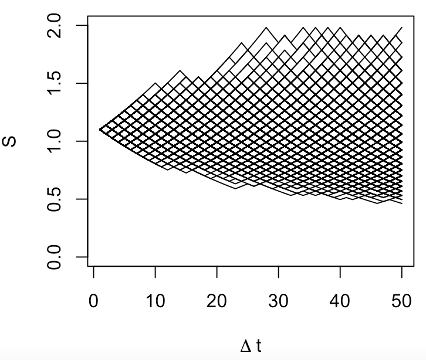
\includegraphics[height=18em]{../imagenes/Imagen 1.png}
\end{frame}

\begin{comment}
  
\subsection{Parte a)}

\begin{frame}{Pregunta 4 Parte a)}
  \justify
  
  \Pregcuatro\\

  \vspace{1em}
  \textbf{a)} \Pregcuatroa
\end{frame}

\subsection{Parte b)}

\begin{frame}{Pregunta 4 Parte b)}
  \justify
  
  \Pregcuatro\\
  
  \vspace{1em}
  \textbf{b)} \Pregcuatrob
\end{frame}

\subsection{Parte c)}

\begin{frame}{Pregunta 4 Parte c)}
  \justify
  
  \Pregcuatro\\

  \vspace{1em}
  \textbf{c} \Pregcuatroc
\end{frame}
\end{comment}

\section{Pregunta 5}
% #region Variables Pregunta 5

% Preguntas
\newcommand{\Pregcinco}{Considere una opción call Americana de una divisa. El valor de la divisa hoy es de \$700, 
el strike Price es de \$710, la tasa libre de riesgo local es del 12\% continua anual 
(la tasa libre de riesgo extranjera es del 4\% continua anual), la volatilidad es del 
40\% anual y la madurez del derivado es de 6 meses. }
\newcommand{\Pregcincoa}{Calcule u, d y p para un árbol binomial de dos pasos.}
\newcommand{\Pregcincob}{Calcule el valor de la opción.}
\newcommand{\Pregcincoc}{Verifique que se obtiene el mismo resultado usando R.}
\newcommand{\Pregcincod}{Calcule el valor de la opción para 5, 50, 100 y 500 pasos (usando R).}
% Fórmulas


% #endregion
\begin{frame}{Pregunta 5}
  \justify
\Pregcinco
\vspace{1em}

\begin{enumerate}[label=\textbf{\alph*)}]
  \item \Pregcincoa
  \item \Pregcincob
  \item \Pregcincoc
  \item \Pregcincod
\end{enumerate}

\end{frame}
\begin{comment}

\subsection{Parte a)}

\begin{frame}{Pregunta 5 Parte a)}
  \justify
  
  \Pregcinco\\

  \vspace{1em}
  \textbf{a)} \Pregcincoa
\end{frame}

\subsection{Parte b)}

\begin{frame}{Pregunta 5 Parte b)}
  \justify
  
  \Pregcinco\\
  
  \vspace{1em}
  \textbf{b)} \Pregcincob
\end{frame}

\subsection{Parte c)}

\begin{frame}{Pregunta 5 Parte c)}
  \justify
  
  \Pregcinco\\
  
  \vspace{1em}
  \textbf{c)} \Pregcincoc
\end{frame}

\subsection{Parte d)}


\begin{frame}{Pregunta 5 Parte d)}
  \justify
  
  \Pregcinco\\
  
  \vspace{1em}
  \textbf{d)} \Pregcincod
\end{frame}
\end{comment}

\end{document}